\chapter{Algoritmos de raiz quadrada}

\index{algoritmo de raiz quadrada}

Um \key{algoritmo de raiz quadrada} é um algoritmo
que possui uma raiz quadrada em sua complexidade de tempo.
Uma raiz quadrada pode ser vista como um "logaritmo do homem pobre":
a complexidade $O(\sqrt n)$ é melhor que $O(n)$
mas pior que $O(\log n)$.
De qualquer forma, muitos algoritmos de raiz quadrada são rápidos e utilizáveis na prática.

Como exemplo, considere o problema de
criar uma estrutura de dados que suporte
duas operações em um array:
modificar um elemento em uma dada posição
e calcular a soma dos elementos no intervalo dado.
Já resolvemos o problema usando
árvores binárias indexadas e árvores de segmentos,
que suportam ambas as operações em tempo $O(\log n)$.
No entanto, agora resolveremos o problema
de outra forma usando uma estrutura de raiz quadrada
que nos permite modificar elementos em tempo $O(1)$
e calcular somas em tempo $O(\sqrt n)$.

A ideia é dividir o array em \emph{blocos}
de tamanho $\sqrt n$ para que cada bloco contenha
a soma dos elementos dentro do bloco.
Por exemplo, um array de 16 elementos será
dividido em blocos de 4 elementos como segue:

\begin{center}
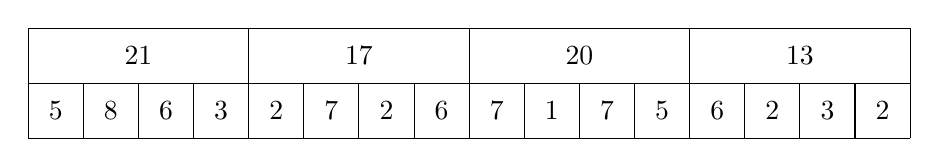
\begin{tikzpicture}[scale=0.7]
\draw (0,0) grid (16,1);

\draw (0,1) rectangle (4,2);
\draw (4,1) rectangle (8,2);
\draw (8,1) rectangle (12,2);
\draw (12,1) rectangle (16,2);

\node at (0.5, 0.5) {5};
\node at (1.5, 0.5) {8};
\node at (2.5, 0.5) {6};
\node at (3.5, 0.5) {3};
\node at (4.5, 0.5) {2};
\node at (5.5, 0.5) {7};
\node at (6.5, 0.5) {2};
\node at (7.5, 0.5) {6};
\node at (8.5, 0.5) {7};
\node at (9.5, 0.5) {1};
\node at (10.5, 0.5) {7};
\node at (11.5, 0.5) {5};
\node at (12.5, 0.5) {6};
\node at (13.5, 0.5) {2};
\node at (14.5, 0.5) {3};
\node at (15.5, 0.5) {2};

\node at (2, 1.5) {21};
\node at (6, 1.5) {17};
\node at (10, 1.5) {20};
\node at (14, 1.5) {13};

\end{tikzpicture}
\end{center}

Nesta estrutura,
é fácil modificar os elementos do array,
pois basta atualizar
a soma de um único bloco
após cada modificação,
o que pode ser feito em tempo $O(1)$.
Por exemplo, a figura a seguir mostra
como o valor de um elemento e
a soma do bloco correspondente mudam:

\begin{center}
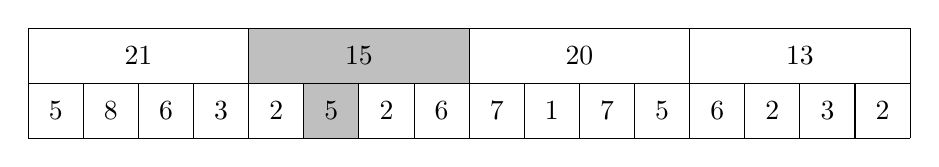
\begin{tikzpicture}[scale=0.7]
\fill[color=lightgray] (5,0) rectangle (6,1);
\draw (0,0) grid (16,1);

\fill[color=lightgray] (4,1) rectangle (8,2);
\draw (0,1) rectangle (4,2);
\draw (4,1) rectangle (8,2);
\draw (8,1) rectangle (12,2);
\draw (12,1) rectangle (16,2);

\node at (0.5, 0.5) {5};
\node at (1.5, 0.5) {8};
\node at (2.5, 0.5) {6};
\node at (3.5, 0.5) {3};
\node at (4.5, 0.5) {2};
\node at (5.5, 0.5) {5};
\node at (6.5, 0.5) {2};
\node at (7.5, 0.5) {6};
\node at (8.5, 0.5) {7};
\node at (9.5, 0.5) {1};
\node at (10.5, 0.5) {7};
\node at (11.5, 0.5) {5};
\node at (12.5, 0.5) {6};
\node at (13.5, 0.5) {2};
\node at (14.5, 0.5) {3};
\node at (15.5, 0.5) {2};

\node at (2, 1.5) {21};
\node at (6, 1.5) {15};
\node at (10, 1.5) {20};
\node at (14, 1.5) {13};

\end{tikzpicture}
\end{center}

Então, para calcular a soma dos elementos em um intervalo,
dividimos o intervalo em três partes, de forma que
a soma consista em valores de elementos individuais
e somas de blocos entre eles:

\begin{center}
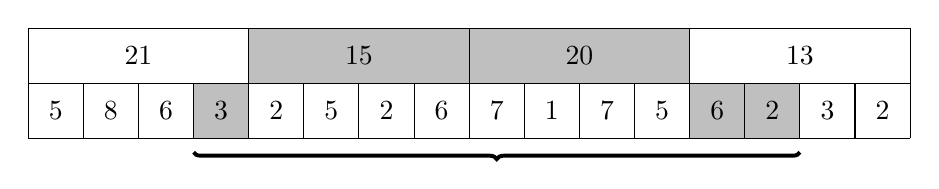
\begin{tikzpicture}[scale=0.7]
\fill[color=lightgray] (3,0) rectangle (4,1);
\fill[color=lightgray] (12,0) rectangle (13,1);
\fill[color=lightgray] (13,0) rectangle (14,1);
\draw (0,0) grid (16,1);

\fill[color=lightgray] (4,1) rectangle (8,2);
\fill[color=lightgray] (8,1) rectangle (12,2);
\draw (0,1) rectangle (4,2);
\draw (4,1) rectangle (8,2);
\draw (8,1) rectangle (12,2);
\draw (12,1) rectangle (16,2);

\node at (0.5, 0.5) {5};
\node at (1.5, 0.5) {8};
\node at (2.5, 0.5) {6};
\node at (3.5, 0.5) {3};
\node at (4.5, 0.5) {2};
\node at (5.5, 0.5) {5};
\node at (6.5, 0.5) {2};
\node at (7.5, 0.5) {6};
\node at (8.5, 0.5) {7};
\node at (9.5, 0.5) {1};
\node at (10.5, 0.5) {7};
\node at (11.5, 0.5) {5};
\node at (12.5, 0.5) {6};
\node at (13.5, 0.5) {2};
\node at (14.5, 0.5) {3};
\node at (15.5, 0.5) {2};

\node at (2, 1.5) {21};
\node at (6, 1.5) {15};
\node at (10, 1.5) {20};
\node at (14, 1.5) {13};

\draw [decoration={brace}, decorate, line width=0.5mm] (14,-0.25) -- (3,-0.25);

\end{tikzpicture}
\end{center}

Como o número de elementos individuais é $O(\sqrt n)$
e o número de blocos também é $O(\sqrt n)$,
a consulta de soma leva tempo $O(\sqrt n)$.
O propósito do tamanho do bloco $\sqrt n$ é
que ele \emph{equilibra} duas coisas:
o array é dividido em $\sqrt n$ blocos,
cada um contendo $\sqrt n$ elementos.

Na prática, não é necessário usar o
valor exato de $\sqrt n$ como parâmetro,
e, em vez disso, podemos usar os parâmetros $k$ e $n/k$, onde $k$ é
diferente de $\sqrt n$.
O parâmetro ideal depende do problema e da entrada.
Por exemplo, se um algoritmo frequentemente passa
pelos blocos, mas raramente inspeciona
elementos individuais dentro dos blocos,
pode ser uma boa ideia dividir o array em
$k < \sqrt n$ blocos, cada um contendo $n/k > \sqrt n$
elementos.

\section{Combinando algoritmos}

Nesta seção, discutimos dois algoritmos de raiz quadrada
que se baseiam na combinação de dois algoritmos em um único algoritmo.
Em ambos os casos, poderíamos usar qualquer um dos algoritmos
sem o outro
e resolver o problema em tempo $O(n^2)$.
No entanto, combinando os algoritmos, o tempo de execução é de apenas $O(n \sqrt n)$.

\subsubsection{Processamento de casos}

Suponha que recebamos uma grade bidimensional
que contém $n$ células.
Cada célula recebe uma letra,
e nossa tarefa é encontrar duas células
com a mesma letra cuja distância seja mínima,
onde a distância entre as células
$(x_1,y_1)$ e $(x_2,y_2)$ é $|x_1-x_2|+|y_1-y_2|$.
Por exemplo, considere a grade a seguir:

\begin{center}
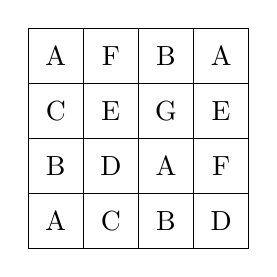
\begin{tikzpicture}[scale=0.7]
\node at (0.5,0.5) {A};
\node at (0.5,1.5) {B};
\node at (0.5,2.5) {C};
\node at (0.5,3.5) {A};
\node at (1.5,0.5) {C};
\node at (1.5,1.5) {D};
\node at (1.5,2.5) {E};
\node at (1.5,3.5) {F};
\node at (2.5,0.5) {B};
\node at (2.5,1.5) {A};
\node at (2.5,2.5) {G};
\node at (2.5,3.5) {B};
\node at (3.5,0.5) {D};
\node at (3.5,1.5) {F};
\node at (3.5,2.5) {E};
\node at (3.5,3.5) {A};
\draw (0,0) grid (4,4);
\end{tikzpicture}
\end{center}
Neste caso, a distância mínima é 2 entre as duas letras 'E'.

Podemos resolver o problema considerando cada letra separadamente.
Usando essa abordagem, o novo problema é calcular
a distância mínima
entre duas células com uma letra \emph{fixa} $c$.
Vamos nos concentrar em dois algoritmos para isso:

\emph{Algoritmo 1:} Percorra todos os pares de células com a letra $c$,
e calcule a distância mínima entre tais células.
Isso levará tempo $O(k^2)$, onde $k$ é o número de células com a letra $c$.

\emph{Algoritmo 2:} Execute uma busca em largura que simultaneamente
começa em cada célula com a letra $c$. A distância mínima entre
duas células com a letra $c$ será calculada em tempo $O(n)$.

Uma maneira de resolver o problema é escolher qualquer um dos
algoritmos e usá-lo para todas as letras.
Se usarmos o Algoritmo 1, o tempo de execução é $O(n^2)$,
porque todas as células podem conter a mesma letra,
e, neste caso, $k=n$.
Também se usarmos o Algoritmo 2, o tempo de execução é $O(n^2)$,
porque todas as células podem ter letras diferentes,
e, neste caso, $n$ buscas são necessárias.

No entanto, podemos \emph{combinar} os dois algoritmos e
usar algoritmos diferentes para letras diferentes,
dependendo de quantas vezes cada letra aparece na grade.
Suponha que uma letra $c$ apareça $k$ vezes.
Se $k \le \sqrt n$, usamos o Algoritmo 1 e, se $k > \sqrt n$,
usamos o Algoritmo 2.
Acontece que, ao fazer isso, o tempo de execução total
do algoritmo é de apenas $O(n \sqrt n)$.

Primeiro, suponha que usamos o Algoritmo 1 para uma letra $c$.
Como $c$ aparece no máximo $\sqrt n$ vezes na grade,
comparamos cada célula com a letra $c$ $O(\sqrt n)$ vezes
com outras células.
Assim, o tempo usado para processar todas essas células é $O(n \sqrt n)$.
Então, suponha que usamos o Algoritmo 2 para uma letra $c$.
Existem no máximo $\sqrt n$ letras assim,
então, processar essas letras também leva tempo $O(n \sqrt n)$.

\subsubsection{Processamento em lote}

Nosso próximo problema também lida com
uma grade bidimensional que contém $n$ células.
Inicialmente, cada célula, exceto uma, é branca.
Realizamos $n-1$ operações, cada uma das quais primeiro
calcula a distância mínima de uma dada célula branca
para uma célula preta e, em seguida, pinta a célula branca de preto.

Por exemplo, considere a seguinte operação:

\begin{center}
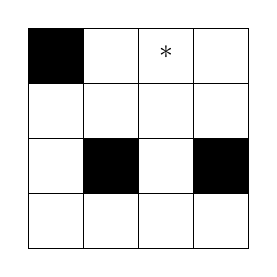
\begin{tikzpicture}[scale=0.7]
\fill[color=black] (1,1) rectangle (2,2);
\fill[color=black] (3,1) rectangle (4,2);
\fill[color=black] (0,3) rectangle (1,4);
\node at (2.5,3.5) {*};
\draw (0,0) grid (4,4);
\end{tikzpicture}
\end{center}

Primeiro, calculamos a distância mínima
da célula branca marcada com * para uma célula preta.
A distância mínima é 2, pois podemos mover
duas casas para a esquerda até uma célula preta.
Então, pintamos a célula branca de preto:

\begin{center}
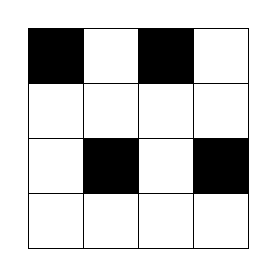
\begin{tikzpicture}[scale=0.7]
\fill[color=black] (1,1) rectangle (2,2);
\fill[color=black] (3,1) rectangle (4,2);
\fill[color=black] (0,3) rectangle (1,4);
\fill[color=black] (2,3) rectangle (3,4);
\draw (0,0) grid (4,4);
\end{tikzpicture}
\end{center}

Considere os dois algoritmos a seguir:

\emph{Algoritmo 1:} Use a busca em largura
para calcular,
para cada célula branca, a distância até a célula preta mais próxima.
Isso leva tempo $O(n)$, e, após a busca,
podemos encontrar a distância mínima de qualquer célula branca
para uma célula preta em tempo $O(1)$.

\emph{Algoritmo 2:} Mantenha uma lista de células que foram
pintadas de preto, percorra essa lista em cada operação
e adicione uma nova célula à lista.
Uma operação leva tempo $O(k)$, onde $k$ é o tamanho da lista.

Combinamos os algoritmos acima
dividindo as operações em
$O(\sqrt n)$ \emph{lotes}, cada um dos quais consiste
em $O(\sqrt n)$ operações.
No início de cada lote,
executamos o Algoritmo 1.
Então, usamos o Algoritmo 2 para processar as operações
no lote.
Limpamos a lista do Algoritmo 2 entre
os lotes.
Em cada operação,
a distância mínima até uma célula preta
é a distância calculada pelo Algoritmo 1
ou a distância calculada pelo Algoritmo 2.

O algoritmo resultante funciona em
tempo $O(n \sqrt n)$.
Primeiro, o Algoritmo 1 é executado $O(\sqrt n)$ vezes,
e cada busca funciona em tempo $O(n)$.
Segundo, ao usar o Algoritmo 2 em um lote,
a lista contém $O(\sqrt n)$ células
(porque limpamos a lista entre os lotes)
e cada operação leva tempo $O(\sqrt n)$.

\section{Partições de inteiros}

Alguns algoritmos de raiz quadrada são baseados na
seguinte observação:
se um inteiro positivo $n$ é representado como
uma soma de inteiros positivos,
tal soma sempre contém no máximo
$O(\sqrt n)$ números \emph{distintos}.
A razão para isso é que, para construir
uma soma que contém um número máximo de elementos distintos,
devemos escolher números \emph{pequenos}.
Se escolhermos os números $1,2,\ldots,k$,
a soma resultante é
\[\frac{k(k+1)}{2}.\]
Assim, a quantidade máxima de números distintos é $k = O(\sqrt n)$.
A seguir, discutiremos dois problemas que podem ser resolvidos
de forma eficiente usando essa observação.

\subsubsection{Mochila}

Suponha que recebamos uma lista de pesos inteiros
cuja soma é $n$.
Nossa tarefa é descobrir todas as somas que podem ser formadas usando
um subconjunto dos pesos. Por exemplo, se os pesos são
$\{1,3,3\}$, as somas possíveis são as seguintes:

\begin{itemize}[noitemsep]
\item $0$ (conjunto vazio)
\item $1$
\item $3$
\item $1+3=4$
\item $3+3=6$
\item $1+3+3=7$
\end{itemize}

Usando a abordagem padrão da mochila (veja o Capítulo 7.4),
o problema pode ser resolvido da seguinte forma:
definimos uma função $\texttt{possível}(x,k)$ cujo valor é 1
se a soma $x$ pode ser formada usando os primeiros $k$ pesos,
e 0 caso contrário.
Como a soma dos pesos é $n$,
existem no máximo $n$ pesos e
todos os valores da função podem ser calculados
em tempo $O(n^2)$ usando programação dinâmica.

No entanto, podemos tornar o algoritmo mais eficiente
usando o fato de que existem no máximo $O(\sqrt n)$
pesos \emph{distintos}.
Assim, podemos processar os pesos em grupos
que consistem em pesos semelhantes.
Podemos processar cada grupo
em tempo $O(n)$, o que resulta em um algoritmo de tempo $O(n \sqrt n)$.

A ideia é usar um array que registre as somas de pesos
que podem ser formadas usando os grupos processados até o momento.
O array contém $n$ elementos: o elemento $k$ é 1 se a soma
$k$ pode ser formada e 0 caso contrário.
Para processar um grupo de pesos, examinamos o array
da esquerda para a direita e registramos as novas somas de pesos que
podem ser formadas usando este grupo e os grupos anteriores.

\subsubsection{Construção de string}

Dada uma string \texttt{s} de tamanho $n$
e um conjunto de strings $D$ cujo tamanho total é $m$,
considere o problema de contar o número de maneiras
pelas quais \texttt{s} pode ser formada como uma concatenação de strings em $D$.
Por exemplo,
se $\texttt{s}=\texttt{ABAB}$ e
$D={\texttt{A},\texttt{B},\texttt{AB}}$,
existem 4 maneiras:

\begin{itemize}[noitemsep]
\item $\texttt{A}+\texttt{B}+\texttt{A}+\texttt{B}$
\item $\texttt{AB}+\texttt{A}+\texttt{B}$
\item $\texttt{A}+\texttt{B}+\texttt{AB}$
\item $\texttt{AB}+\texttt{AB}$
\end{itemize}

Podemos resolver o problema usando programação dinâmica:
seja $\texttt{contagem}(k)$ o número de maneiras de construir o prefixo
$\texttt{s}[0 \ldots k]$ usando as strings em $D$.
Agora, $\texttt{contagem}(n-1)$ fornece a resposta ao problema,
e podemos resolver o problema em tempo $O(n^2)$
usando uma estrutura trie.

No entanto, podemos resolver o problema de forma mais eficiente
usando hashing de strings e o fato de haver
no máximo $O(\sqrt m)$ tamanhos de string distintos em $D$.
Primeiro, construímos um conjunto $H$ que contém todos
os valores de hash das strings em $D$.
Então, ao calcular um valor de $\texttt{contagem}(k)$,
percorremos todos os valores de $p$,
de forma que haja uma string de tamanho $p$ em $D$,
calculamos o valor de hash de $\texttt{s}[k-p+1 \ldots k]$
e verificamos se ele pertence a $H$.
Como existem no máximo $O(\sqrt m)$ tamanhos de string distintos,
isso resulta em um algoritmo cujo tempo de execução é $O(n \sqrt m)$.

\section{Algoritmo de Mo}

\index{algoritmo de Mo}

O \key{algoritmo de Mo}\footnote{De acordo com \cite{cod15}, este algoritmo
tem o nome de Mo Tao, um programador competitivo chinês, mas
a técnica já apareceu antes na literatura \cite{ken06}.}
pode ser usado em muitos problemas
que exigem o processamento de consultas de intervalo em
um array \emph{estático}, ou seja, os valores do array
não mudam entre as consultas.
Em cada consulta, recebemos um intervalo $[a,b]$,
e devemos calcular um valor com base nos
elementos do array entre as posições $a$ e $b$.
Como o array é estático,
as consultas podem ser processadas em qualquer ordem,
e o algoritmo de Mo
processa as consultas em uma ordem especial que garante
que o algoritmo funcione de forma eficiente.

O algoritmo de Mo mantém um \emph{intervalo ativo}
do array, e a resposta a uma consulta
referente ao intervalo ativo é conhecida a cada momento.
O algoritmo processa as consultas uma a uma,
e sempre move as extremidades do
intervalo ativo inserindo e removendo elementos.
A complexidade de tempo do algoritmo é
$O(n \sqrt n f(n))$, em que o array contém
$n$ elementos, há $n$ consultas
e cada inserção e remoção de um elemento
leva tempo $O(f(n))$.

O truque no algoritmo de Mo é a ordem
em que as consultas são processadas:
O array é dividido em blocos de $k=O(\sqrt n)$
elementos, e uma consulta $[a_1,b_1]$
é processada antes de uma consulta $[a_2,b_2]$,
se
\begin{itemize}
\item $\lfloor a_1/k \rfloor < \lfloor a_2/k \rfloor$ ou
\item $\lfloor a_1/k \rfloor = \lfloor a_2/k \rfloor$ e $b_1 < b_2$.
\end{itemize}

Assim, todas as consultas cujas extremidades esquerdas estão
em um determinado bloco são processadas uma após a outra,
ordenadas de acordo com suas extremidades direitas.
Usando essa ordem, o algoritmo
só executa $O(n \sqrt n)$ operações,
porque a extremidade esquerda se move
$O(n)$ vezes $O(\sqrt n)$ etapas,
e a extremidade direita se move
$O(\sqrt n)$ vezes $O(n)$ etapas. Assim, ambas
as extremidades se movem um total de $O(n \sqrt n)$ etapas durante o algoritmo.

\subsubsection*{Exemplo}

Como exemplo, considere um problema
onde recebemos um conjunto de consultas,
cada uma delas correspondendo a um intervalo em um array,
e nossa tarefa é calcular, para cada consulta,
o número de elementos \emph{distintos} no intervalo.

No algoritmo de Mo, as consultas são sempre classificadas
da mesma maneira, mas depende do problema
como a resposta à consulta é mantida.
Neste problema, podemos manter um array
\texttt{contagem}, em que $\texttt{contagem}[x]$
indica o número de vezes que um elemento $x$
ocorre no intervalo ativo.

Quando passamos de uma consulta para outra,
o intervalo ativo muda.
Por exemplo, se o intervalo atual for
\begin{center}
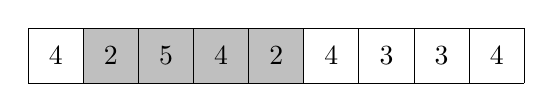
\begin{tikzpicture}[scale=0.7]
\fill[color=lightgray] (1,0) rectangle (5,1);
\draw (0,0) grid (9,1);
\node at (0.5, 0.5) {4};
\node at (1.5, 0.5) {2};
\node at (2.5, 0.5) {5};
\node at (3.5, 0.5) {4};
\node at (4.5, 0.5) {2};
\node at (5.5, 0.5) {4};
\node at (6.5, 0.5) {3};
\node at (7.5, 0.5) {3};
\node at (8.5, 0.5) {4};
\end{tikzpicture}
\end{center}
e o próximo intervalo for
\begin{center}
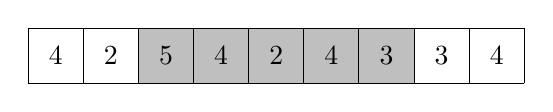
\begin{tikzpicture}[scale=0.7]
\fill[color=lightgray] (2,0) rectangle (7,1);
\draw (0,0) grid (9,1);
\node at (0.5, 0.5) {4};
\node at (1.5, 0.5) {2};
\node at (2.5, 0.5) {5};
\node at (3.5, 0.5) {4};
\node at (4.5, 0.5) {2};
\node at (5.5, 0.5) {4};
\node at (6.5, 0.5) {3};
\node at (7.5, 0.5) {3};
\node at (8.5, 0.5) {4};
\end{tikzpicture}
\end{center}
haverá três etapas:
a extremidade esquerda se move uma etapa para a direita,
e a extremidade direita se move duas etapas para a direita.

Após cada etapa, o array \texttt{contagem}
precisa ser atualizado.
Após adicionar um elemento $x$,
aumentamos o valor de
$\texttt{contagem}[x]$ em 1,
e, se $\texttt{contagem}[x]=1$ depois disso,
também aumentamos a resposta à consulta em 1.
Da mesma forma, após remover um elemento $x$,
diminuímos o valor de
$\texttt{contagem}[x]$ em 1,
e, se $\texttt{contagem}[x]=0$ depois disso,
também diminuímos a resposta à consulta em 1.

Neste problema, o tempo necessário para executar
cada etapa é $O(1)$, então a complexidade de tempo total
do algoritmo é $O(n \sqrt n)$.